\section{System's Perspective}

\subsection{Design and Architecture of MiniTwit}
The MiniTwit system is designed in a way that allows us to separate the models, the views and the controllers,
as seen in figure \ref{fig:minitwit}. This is done to reduce the coupling between our components and to make 
it simpler to extend the functionality of the application. For both safety and simplification of CRUD operations we used Gorm.

\begin{figure}[H]
    \centering
    \captionsetup{justification=centering,margin=1cm}
    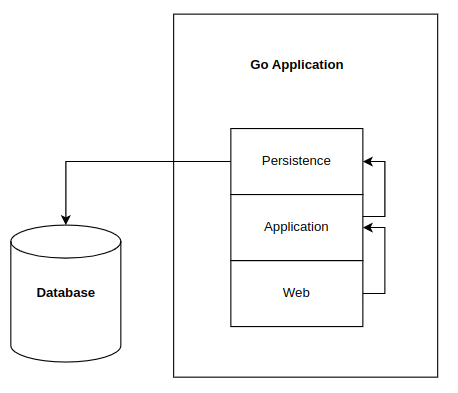
\includegraphics[width=0.8\linewidth]{report/images/system_architecture.png}
    \caption{MiniTwit Architecture}
    \label{fig:minitwit}
\end{figure}

The application is implemented using the RESTful API, which means that when a user interacts with a part of the 
view, an HTTP request containing a new state of the application is sent. This request is then handled by the corresponding controller, and it ensures 
that the correct action is taken. This could be a call to a function that updates the model, and the return of 
an appropriate HTTP response. 


\subsection{Dependencies of MiniTwit system}

For the MiniTwit application to run we are depending on first and foremost Digital Oecan whos servers the application is 
hosted on. The servers are running 9 docker containers responsible for: 
\begin{itemize}
    \item The Database running on a postgres:14.1-alpine image - Responsible for holding all the users data.
    \item The Server itself running on a golang:bullseye image.
    \item A reddis server for storing sessions and the integer 'latest'.
    \item Elastic Search - Indexing logs such that we can search and analyse them
    \item Filebeat for collecting and forwarding the logging to Elastic search
    \item Kibana for visualizing the results from Elastic search
    \item Prometheus for monitoring the application in terms of CPU usage and request time
    \item Grafana for visualizing the monitoring
    \item Nginx for load balancer? skriv her
\end{itemize}

From within each of these containers we depend on large number of libraries of which the major ones we consider to be:
\begin{itemize}
    \item Gorm used for object-relational mapping allowing us to perform CRUD operations io GO.
    \item Gin handling all of the routing of the HTTP methods.
    \item x/crypto/bcrypt libaray for hashing the user password.
\end{itemize}

In a more board term of sense we also depend on Docker, Go and SSH protocol to work. We choose Go for the reason being 
that \todo{skriv her} 

At last we also depend on pre-build git workflows such as \textit{docker/build-push-action@v2} or \textit{rymndhng/release-on-push-action@master}.
\subsubsection{Arguments for ORM and DBMS}

%OBS MSc students: Remember to log and provide good arguments for the choice of ORM framework and chosen DBMS.
In regards to choosing ORM(Object-relational mapping) and DBMS(Database Management Systems) we settled on using \textit{PostgresSQL} as our DBMS and \textit{Gorm} for ORM. In terms of choosing DBMS we considered \textit{SQLite} and \textit{digital ocean manged db}:
\begin{itemize}
    \item Potential arguments over SQLite 
    \begin{itemize}
        \item Scalability
        \item Concurrency
        \item No user management
        \item Network access        
    \end{itemize}
    \item Potential arguments over e.g. digital ocean manged db
    \begin{itemize}
        \item Cost
    \end{itemize}
\end{itemize}

For ORM we considered \textit{XORM}

%OBS MSc students: Remember to log and provide good arguments for the choice of programming language and framework
\subsubsection{Arguments for programming language and framework}

We initially set out to use FastAPI in Python, but eventually settled on GO for multiple reasons. From a personal development perspective, learning a new language is rarely a poor choice. Go is well-known for being relatively fast to learn, whilst maintaining speed. From a more technical perspective Go has advantages over many languages. It's fast, it has concurrency built-in, and it has a strong standard library support, with most important features, even templating, being available as a standard package.

Gin is not the fastest Go framework, but it has several advantages. It is well-maintained, has over twice the amount of github stars than the next most popular framework, and is one of the faster go web frameworks.

Whilst implementing the application in fastAPI might have been faster and easier, due to both prior python knowledge, and general simplicity, the advantages of using go with the GIN framework can't be overstated. 

%OBS MSc students: Remember to log and provide good arguments for the choice of virtualization techniques and deployment targets

Docker was chosen because it's the industry standard. Other container strategies are good, but given knowledge of future need for orchestration (in either docker swarm or kubernetes) Docker was an obvious choice.  (ok I guess man også kunne bruge podman med kubernetes)

We used Digital Ocean mainly for budgetary reasons and for ease of deployement. Using the Github Student Starter pack, \$200 in free credits were made available to us. This was enough to ensure that the application was able to run for the duration of the course. In fact it allowed us to test out the grander deployment strategies we settled on in the final application; running 7 concurrent droplets. Using multiple accounts furthermore allowed us to create a parallel  


Digital ocean was employed for budgetary reasons, and also because the guides were made for it.
It's also more accessible than other more complicated providers such as AWS. 

% Argue for Terraform choice??

- Infrastructure as code is important for maintainability reasons. Therefore Terraform was an obvious choice.
Terraform is for remote cloud providers. Vagrant is for local development. 
%%% NOTE:
%The application is hosted at Digital Ocean. We use Docker Swarms to scale the application horizontally. For 
%monitoring the application we use Grafana. Logging is done using Elastic Search and Kibana. Additionally, we have a Redis database 
%that stores sessions and the integer 'latest' and a postgreSQL database storing other information, such as 
%the registered users and created messages. 

\subsection{Important Interactions of Subsystems}

\subsection{Current state of the system}

\subsection{Project License}
